\clearpage

\def\chaptertitle{Methodology}

\lhead{\emph{\chaptertitle}}

\chapter{\chaptertitle}
\label{ch:methodology}

Based on the overview of and challenges faced by edge computing paradigms in conforming to SLA constraints, the stated research questions, and the related works discussed above, a hybrid auto-scaling algorithm to answer these questions was proposed during the course of this research project.\par

In this chapter, Section~\ref{sec:ch4-problem-overview} will discuss and formulate the problem of auto-scaling resources on the edge architecture in an SLA-compliant manner. Section~\ref{sec:ch4-hybrid-autoscale-overview} will then detail the high-level overview of the proposed hybrid autoscaler, the objectives of the various algorithm subsystems, the challenges it faces, and an analysis of the algorithm's space and time complexity.

\section{Problem Overview}
\label{sec:ch4-problem-overview}

Edge architectures are split into three layers~\cite{hamdan2020edge}. 
The cloud layer is similar to cloud-computing paradigms, wherein it manages the entire network architecture and stores large scale data. The edge layer consists of smaller scale user data storage and communication with user devices. Finally, the device layer consists of all the user devices that will interact with the edge architecture.\par

\begin{figure}[htb]
    \centering
    \caption{Autoscaling problem overview}
    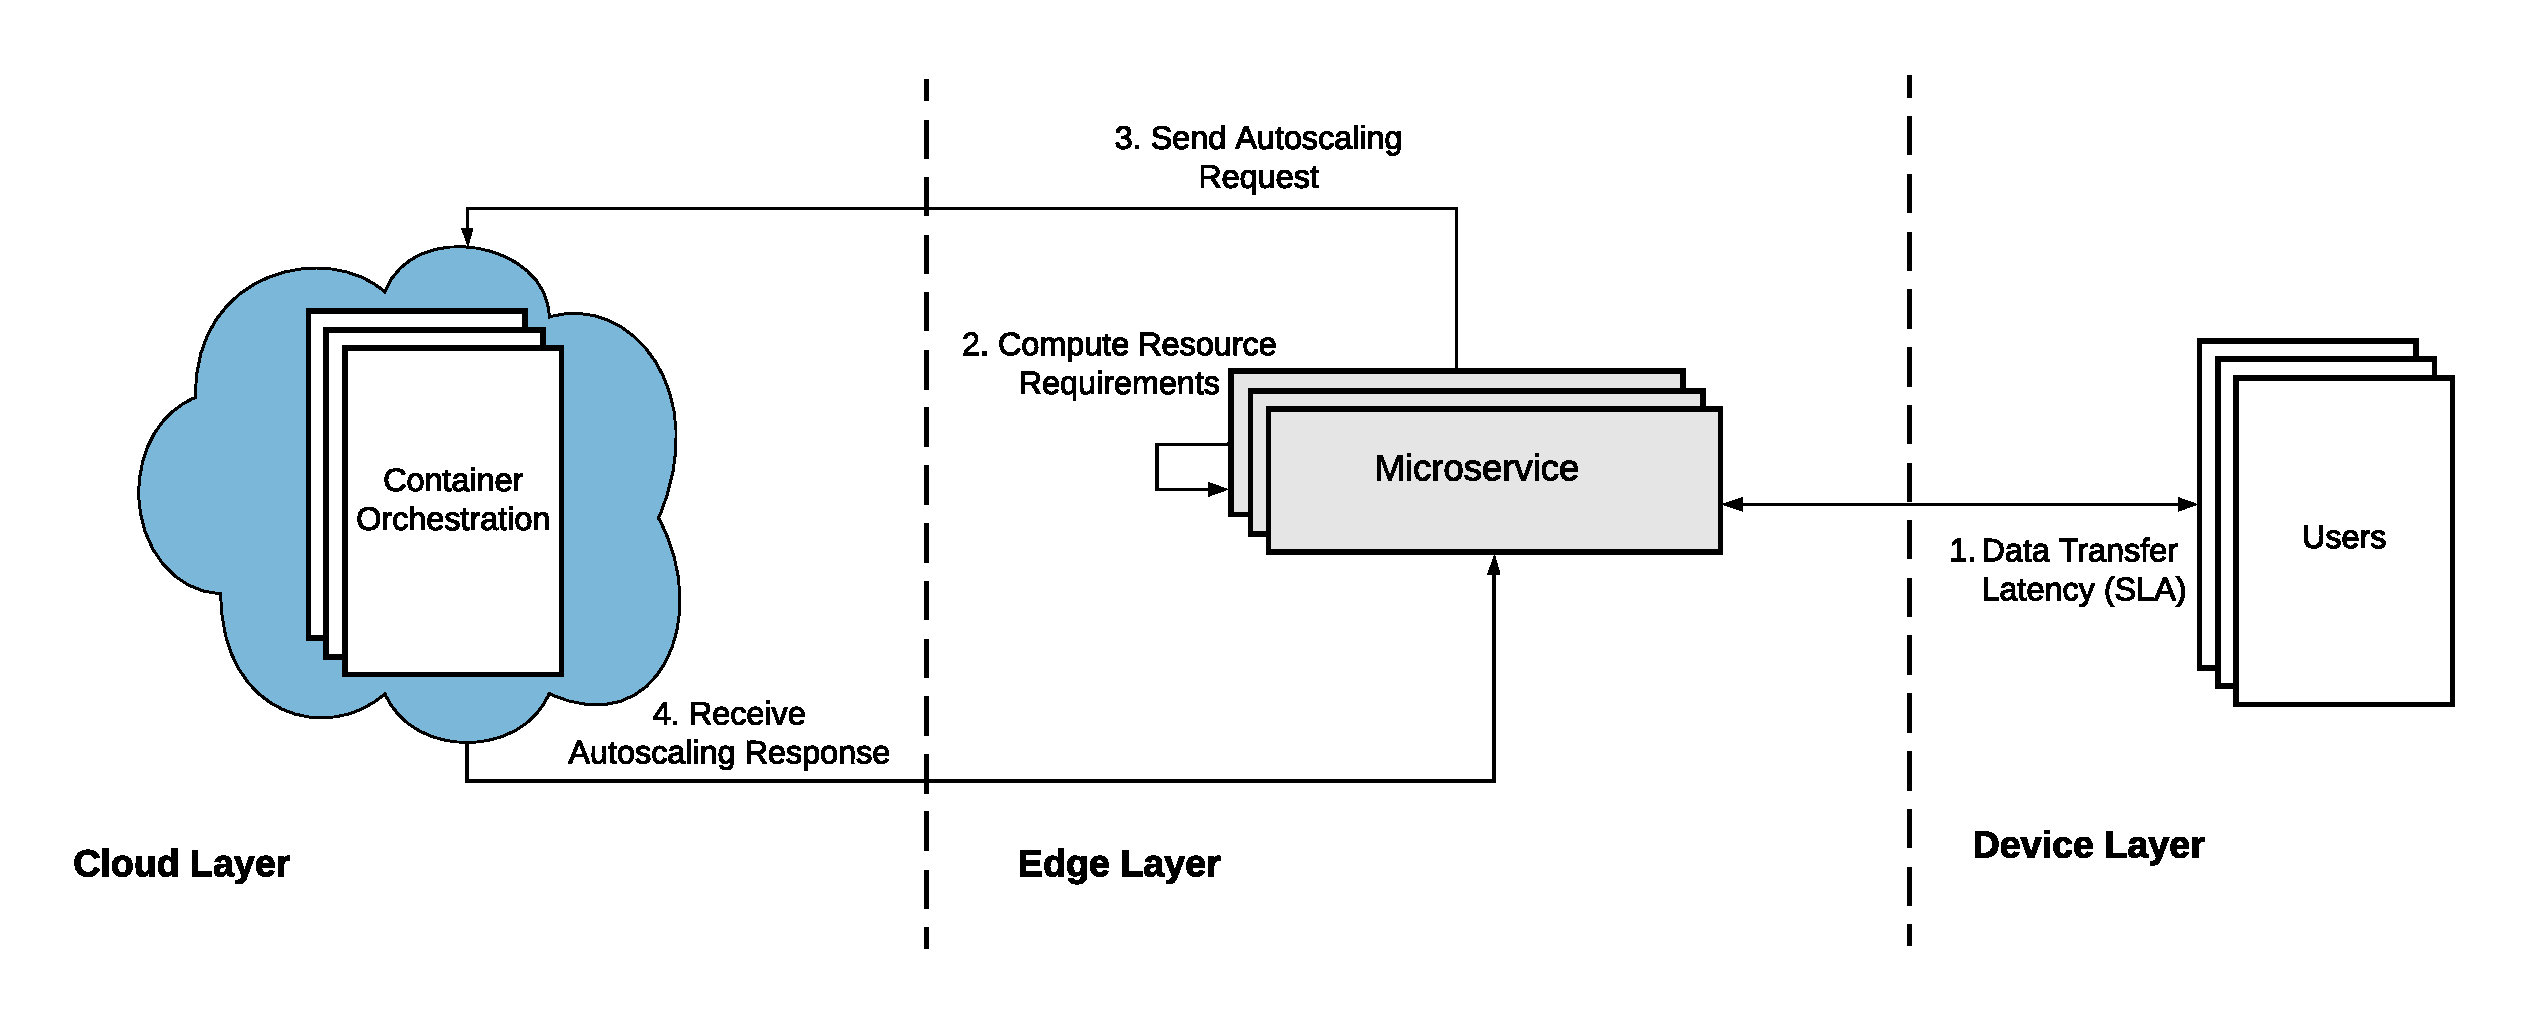
\includegraphics[width=1.0\linewidth]{Figures/Problem-Overview.pdf}
    \label{fig:autoscaling-problem-overview}
\end{figure}

The cloud layer has the most amount of resources allocated to it, which it requires when managing the entire network, computing the intensive processing of large-scale data, and coordinating the resource allocation of the edge layer. However, the primary drawback is the distance between the user and the cloud layer which results in significant latency, making it unsuitable for serving real-time user requests. Thus only system-critical applications such as the controller orchestration control plane are deployed on this layer. The edge layer has far fewer resources than the cloud layer, but its proximity to the users results in lower network latency, making it ideal for resource scaling. For this reason, the edge layer consists of the orchestration tool's worker nodes and the micro-service which receives and serves user data. These worker nodes allocate resources to the micro-service deployments dynamically according to user requirements through the process known as auto-scaling.\par

Figure~\ref{fig:autoscaling-problem-overview} shows the auto-scaling process. The users in the device layer send requests and receive responses to the micro-service deployment in the edge layer. The time taken to receive this response is considered to be the SLA latency metric negotiated between the edge deployment provider and the customer. Using the number of requests being received by the user layer, the edge layer micro-service autoscaler computes the total resource requirements to serve the customer. Based on its findings, the edge layer requests the container orchestration in the cloud layer to either downscale or upscale its resources. The container orchestration then computes the required resource allocation as well as the nodes on which to allocate them and sends its response back to the edge layer.\par

\subsection{Problem Formulation}
\label{subsec:ch4-problem-formulation}

%TC:ignore
\begin{table}
    \caption{Definition of Symbols}\label{tab:symbol-definitions}
    \centering
    \begin{tabular}{rl}
        \toprule
        \textbf{Symbol} & \multicolumn{1}{c}{\textbf{Definition}}\\
        \midrule
        $\mathcal{S}_{c}(t)$ & SLA constraint metric value at time $t$\\
        $\Delta$ & Max SLA metric threshold agreed by the cloud provider \& customer\\
        $\mathcal{V}$ & Number of SLA violations for the chosen metric\\
        $\mathcal{C}_{t}$ & ``Cold start'' time taken to scale resource replicas\\
        $req_{RT}(t)$ & Round trip latency of user request to edge layer\\
        $\mathcal{K}_{t}$ & Constant latency present between edge and device layers\\
        $\mathcal{U}(t)$ & Latency of deployment with unitary resource replica\\
        $\mathcal{D}$ & Total resources in micro-service deployment\\
        $p_{i}$ & Resource pod $i$ of deployment $\mathcal{D}$ where $i = \{1, 2, .. N\}$\\
        $\alpha$ & Cost per unit resource for cloud provider\\
        $\mathcal{L}$ & Maximum allowed deployment cost assigned by the user\\
        $\mathcal{R}(t)$ & Time taken to scale replica resources\\
        \toprule
    \end{tabular}
\end{table}
%TC:endignore

Cloud deployments provide several Quality of Service (QoS) metrics when considering SLA negotiations~\cite{serrano2016sla}. These can be broadly classified into the following four categories:

\begin{itemize}
    \item \textbf{Performance}: These are metrics such as the \textit{response time} which computes the total time taken for a user request to be processed, or the \textit{throughput}, which shows the cloud scalability.
    \item \textbf{Availability}: These include the \textit{abandon rate} which shows the ratio of dropped service requests to the total user requests, and the \textit{use rate} which calculates the amount of time a cloud service was used. Furthermore, certain performance metrics such as \textit{response time} exceeding their thresholds can be considered availability metrics as well.
    \item \textbf{Reliability}: This includes metrics such as the \textit{mean failure time} which calculates the predicted time between service failures, and the \textit{mean recovery time} which is the average time it takes for the service to recover from said failure.
    \item \textbf{Cost}: This includes \textit{financial} costs of deploying or using a cloud service, as well as \textit{energy} costs which compute the carbon footprint of running a cloud service.
\end{itemize}

For this research, we utilize the performance metric \textit{response time} of the user requests as the SLA constraint metric. This metric was chosen due to it being affected the most by intelligently auto-scaling cloud services. Reliability and cost metrics such as \textit{energy} do not correlate well to auto-scaling, while availability metrics such as \textit{abandon rate} are too vague in their reading, showing a binary value of the request either being dropped, or processed. By using this metric, the cloud deployment guaranteed that all requests would be served under a certain threshold.

For real-time applications, the auto-scaling should adhere to the SLA metric as much as possible, and try to minimize the number of violations. An SLA constraint $\mathcal{S}_{c}(t)$ is defined as a metric value not exceeding above a threshold $\Delta$ agreed by both the cloud provider and the customer.

\begin{equation}
    \mathcal{S}_{c}(t) > \Delta
    \label{eqn:sla-threshold}
\end{equation}

The threshold $\Delta$ shown in Equation~\ref{eqn:sla-threshold} varies from application to application. Hussain \textit{et al}.~\cite{hussain2016sla} provided a framework wherein multiple SLA thresholds were configured by the cloud provider and customer, so as to apply them for a variety of use cases, and to ensure differing responses based on the severity of the violation. For a response time latency based metric, these thresholds can broadly be classified into three categories.

\begin{itemize}
    \item \textbf{Flexible}: This is typically the highest allowed violation threshold for the application. Flexible SLA metrics are used to gauge the availability of the deployment. Most IoT applications employ this threshold.
    \item \textbf{Moderate}: This threshold is a trade-off between flexible and stricter SLA thresholds. This threshold is used by applications to ensure a real-time capability such as traffic light scheduling in railways.
    \item \textbf{Strict}: This is the lowest allowed violation threshold in the application. This threshold is significantly challenging to maintain and is used by extremely time-critical applications such as remote-controlled tools for medical surgeries.
\end{itemize}

The auto-scaling will thus use a resource metric to scale its resources up or down. The autoscaler will check to see if the micro-service metric exceeds the threshold for a certain time period, and if so, autoscale resources accordingly. A problem arises in the time it takes to scale these resources, however. This time to increase the number of resource replicas $\mathcal{R}$, which we define as the cold start time $\mathcal{C}(t)$ which can be defined as:

\begin{equation}
    \mathcal{C}(t) = \mathcal{R}_{download}(t) + \mathcal{R}_{deploy}(t) + \mathcal{R}_{register}(t)
\end{equation}

Here, the cold start time $\mathcal{C}(t)$ is defined as the summation of the time taken for the replica $\mathcal{R}$ to be downloaded, deployed on the data plane, and registered with the control plane for scheduling and accepting user requests. The replica image is typically downloaded from a public repository. This download time is usually a one-time delay due to optimizations done on modern container orchestration software, and can be ignored for SLA latency calculations. Using this information, we can reduce this equation to the following:

\begin{equation}
    \mathcal{C}(t) \approx \mathcal{R}_{deploy}(t) + \mathcal{R}_{register}(t)
\end{equation}


Here, the time to deploy and register the replica to the container orchestration cloud layer cannot be avoided. Furthermore, it can be shown that the number of SLA violations $\mathcal{V} \propto \mathcal{C}(t)$ due to the correlation between cold-start delay and the lack of available resources~\cite{patel2021systematic}.\par

Thus, when computing the SLA constraint value for a latency metric, the SLA latency can be re-written as the sum of the cold-start time and the round-trip time taken for the request.

\begin{equation}
    \mathcal{S}_{c}(t) = \mathcal{C}(t) + req_{RT}(t)
\end{equation}


This round-trip time $req_{RT}(t)$ is the combined sum of the inherent delay present in the network layer $latency_{N/W}(t)$, and the time taken for the edge application to process the request $processing_{app}(t)$.

\begin{equation}
    req_{RT}(t) = 2 \times latency_{N/W}(t) + processing_{app}(t)
\end{equation}

The network delay can be reduced by investing in higher network bandwidths, but such improvements have a maximum physical limit, which would not solve the cold start issue. Here we consider this latency to be a constant $\mathcal{K}(t)$. Furthermore, $processing_{app}(t)$ is inversely proportional to the available resources to the application $\mathcal{D}$, since increasing the number of resource replicas helps spread out the user request workload thus reducing the chances of a bottleneck. Using this information, $req_{RT}(t)$ can be approximated as:

\begin{equation}
    req_{RT}(t) \approx \mathcal{K}(t) + \cfrac{\mathcal{U}(t)}{\mathcal{D}}
\end{equation}

Where $\mathcal{U}(t)$ is the maximum latency of a unitary resource deployment. For horizontal pod auto-scaling, the resources here are the number of pods in deployment resources $\mathcal{D}$ such that $\mathcal{D} = \sum_{i} p_{i}$, where $i$ represents the current number of active pods. These pods are the smallest unit of resource for auto-scaling purposes that process the user requests. The final SLA equation can be re-written as follows:

\begin{equation}
    \mathcal{S}_{c}(t) = \mathcal{C}(t) + \cfrac{\mathcal{U}(t)}{\sum_{i} p_{i}} + \mathcal{K}(t)
    \label{eqn:sla-cold-start}
\end{equation}

Thus, the primary aim of the autoscaler is to significantly reduce or even eliminate the cold start, while also increasing the number of resources assigned to the deployment to minimize the application latency. By doing so, the autoscaler aims to reduce the SLA latency below the agreed threshold $\Delta$ thus minimizing the number of SLA violations $\mathcal{V}$.\par

From the above equation, it is clear that $\lim_{\sum_{i} p_{i} \to \infty} \cfrac{\mathcal{U}(t)}{\sum_{i} p_{i}} = 0$.

%\tawfiq{you may use the following to make the above argument more fancy :)}
%$\lim_{\sum_{i} p_{i} \to \infty} \frac{\mathcal{U}(t)}{\sum_{i} p_{i}} = 0$

Thus, the equation incentivizes ignoring intelligently auto-scaling altogether and simply allocate the maximum number of pods to the deployment. However, there are drawbacks to doing so.\par

Most cloud providers such as Amazon Web Services and Google Cloud Platform allocate a cost for each resource assignment to the deployment. If the maximum number of pods that can be deployed is $N$, the cost is calculated as follows.

\begin{equation}
    cost = \alpha \times \sum_{i} p_{i} \quad ;\,i \le N
    \label{eqn:cost}
\end{equation}

Where $\alpha$ is the unitary resource cost which may vary depending on the cloud provider. Thus, simply scaling all resources to the maximum amount may result in substantial and infeasibly high deployment costs. Based on this additional information, the auto-scaling SLA Equation~\ref{eqn:sla-cold-start} and the cost Equation~\ref{eqn:cost} can be merged to form an optimization problem $\mathcal{P}$.

\begin{equation}
    \mathcal{P} = x \times \mathcal{S}_{c}(t) + y \times cost
    \label{eqn:optimization-problem}
\end{equation}

The objective of the autoscaler is to assign resources in a way that minimizes both the latency, as well as the cost, thus minimizing $\mathcal{P}$. The parameters $x$ and $y$ dictate how important cost and latency are relative to each other when considering auto-scaling. For this research, we will configure these values as $x = y = 0.5$, implying both are equally important. Furthermore, the customer will have a maximum ``budget'' $\mathcal{L}$ which the deployment must not exceed. Maximizing the value of the resources in $\mathcal{D}$ while limiting the cost below the threshold $\mathcal{L}$ to reduce the SLA constraint metric $\mathcal{S}_{c}$ below the agreed threshold is akin to the famous Knapsack Problem~\cite{martello1987algorithms}. This problem is proven to be NP-Hard, and as such no known algorithm can determine the best value in polynomial time as demonstrated by Kellerer \textit{et al}.~\cite{kellerer2004introduction}. However, an approximation close to this best value can be computed instead, and this can be done in polynomial time. Due to this, most autoscalers rely on a reactive rule-based or proactive machine-learning technique to compute such close approximations.\par

A problem however arises in the amount of resources it takes to train a proactive model. Not only does the training process consume a significant amount of CPU and memory resources, but it also requires a large time-series dataset. This dataset is necessary to generate a sufficient number of training windows. Without enough training windows, the model will produce erroneous results. While hybrid models help to mitigate the initial errors via the reactive auto-scaling component, the questions regarding the proactive model's resource usage remain an open issue~\cite{radhika2021review}.\par

%Another issue in proactive autoscalers is that not only does it predict increases in utilization before-hand, it also does so for the drop-off in utilization. This can lead to the edge deployment prematurely reducing its resources due to the drop-off forecast, causing several SLA violations due to low availability of resources. To offset this, several hybrid algorithms combine the readings of their reactive and proactive autoscalers, and autoscale according to the highest reading. While this approach works, such algorithms render the accurate resource drop-off predictions of the forecaster redundant, merely taking up precious computation space in the edge deployment.\par

Another issue in a purely proactive autoscaler is the amount of time it takes to both train the model, as well as generate the predictions. Torres \textit{et al}.~\cite{torres2021deep} have demonstrated that time-series forecasters such as LSTM and ARIMA are known to typically have incredibly complex deep neural networks with thousands of neurons in several layers. They demonstrated that even when running such a deep neural network on a cloud architecture, with the aid of 6 cores of CPU and 16 GB of memory resources, and additional parallelization through the use of modern graphical processing units (GPU), this can result in the training process taking upwards of an hour. A large training time makes it incredibly difficult to actively tune the hyper-parameters of the model based on the perceived accuracy, as adapting these values too frequently would result in several hours of training per day, during which the model is unable to predict new values. Once again, a hybrid architecture is typically used to mitigate this issue, as when the proactive model is training, the reactive autoscaler takes over. However, this approach is not feasible for an SLA-constrained architecture, as the reactive component is not SLA-compliant due to its inability to mitigate the cold start problem.\par


In most proactive autoscalers, the forecaster attempts to accurately model the time-series curve to allocate resources effectively. Even in the hybrid algorithms that have been proposed in Section~\ref{sec:ch3-hybrid-solutions}, the proactive modules of the autoscalers are generally unmodified proactive forecasters bundled together with a reactive component. This strategy of attempting to perfectly forecast the curve is what takes such large amounts of resources.\par

Hence, the autoscaler proposed in this thesis will not attempt to predict the exact resource workload. Instead, the time-series graph is heavily simplified using a noise filtering method and then inputted to the machine learning model. Furthermore, the time-series forecaster only attempts to predict the exact timestamp when resource requirements start to increase. Every other requirement, such as the stable resource utilization, as well as the drop-off in non-peak time periods can be handled by the reactive autoscaler, thus heavily simplifying the forecaster architecture. This drastically reduces the forecaster training time to a few minutes. The simplified forecaster has the additional benefit of not requiring incredibly lengthy amounts of time-series data to be stored for it to make accurate predictions, thus this data can also be kept in the edge layer. This makes the autoscaler extremely lightweight, responsive, and most importantly SLA-compliant, thus making it capable of being deployed in an edge environment.\par

\section{Proposed Hybrid Autoscaler}
\label{sec:ch4-hybrid-autoscale-overview} 

\begin{figure}[htb]
    \centering
    \caption{Proposed hybrid architecture overview}
    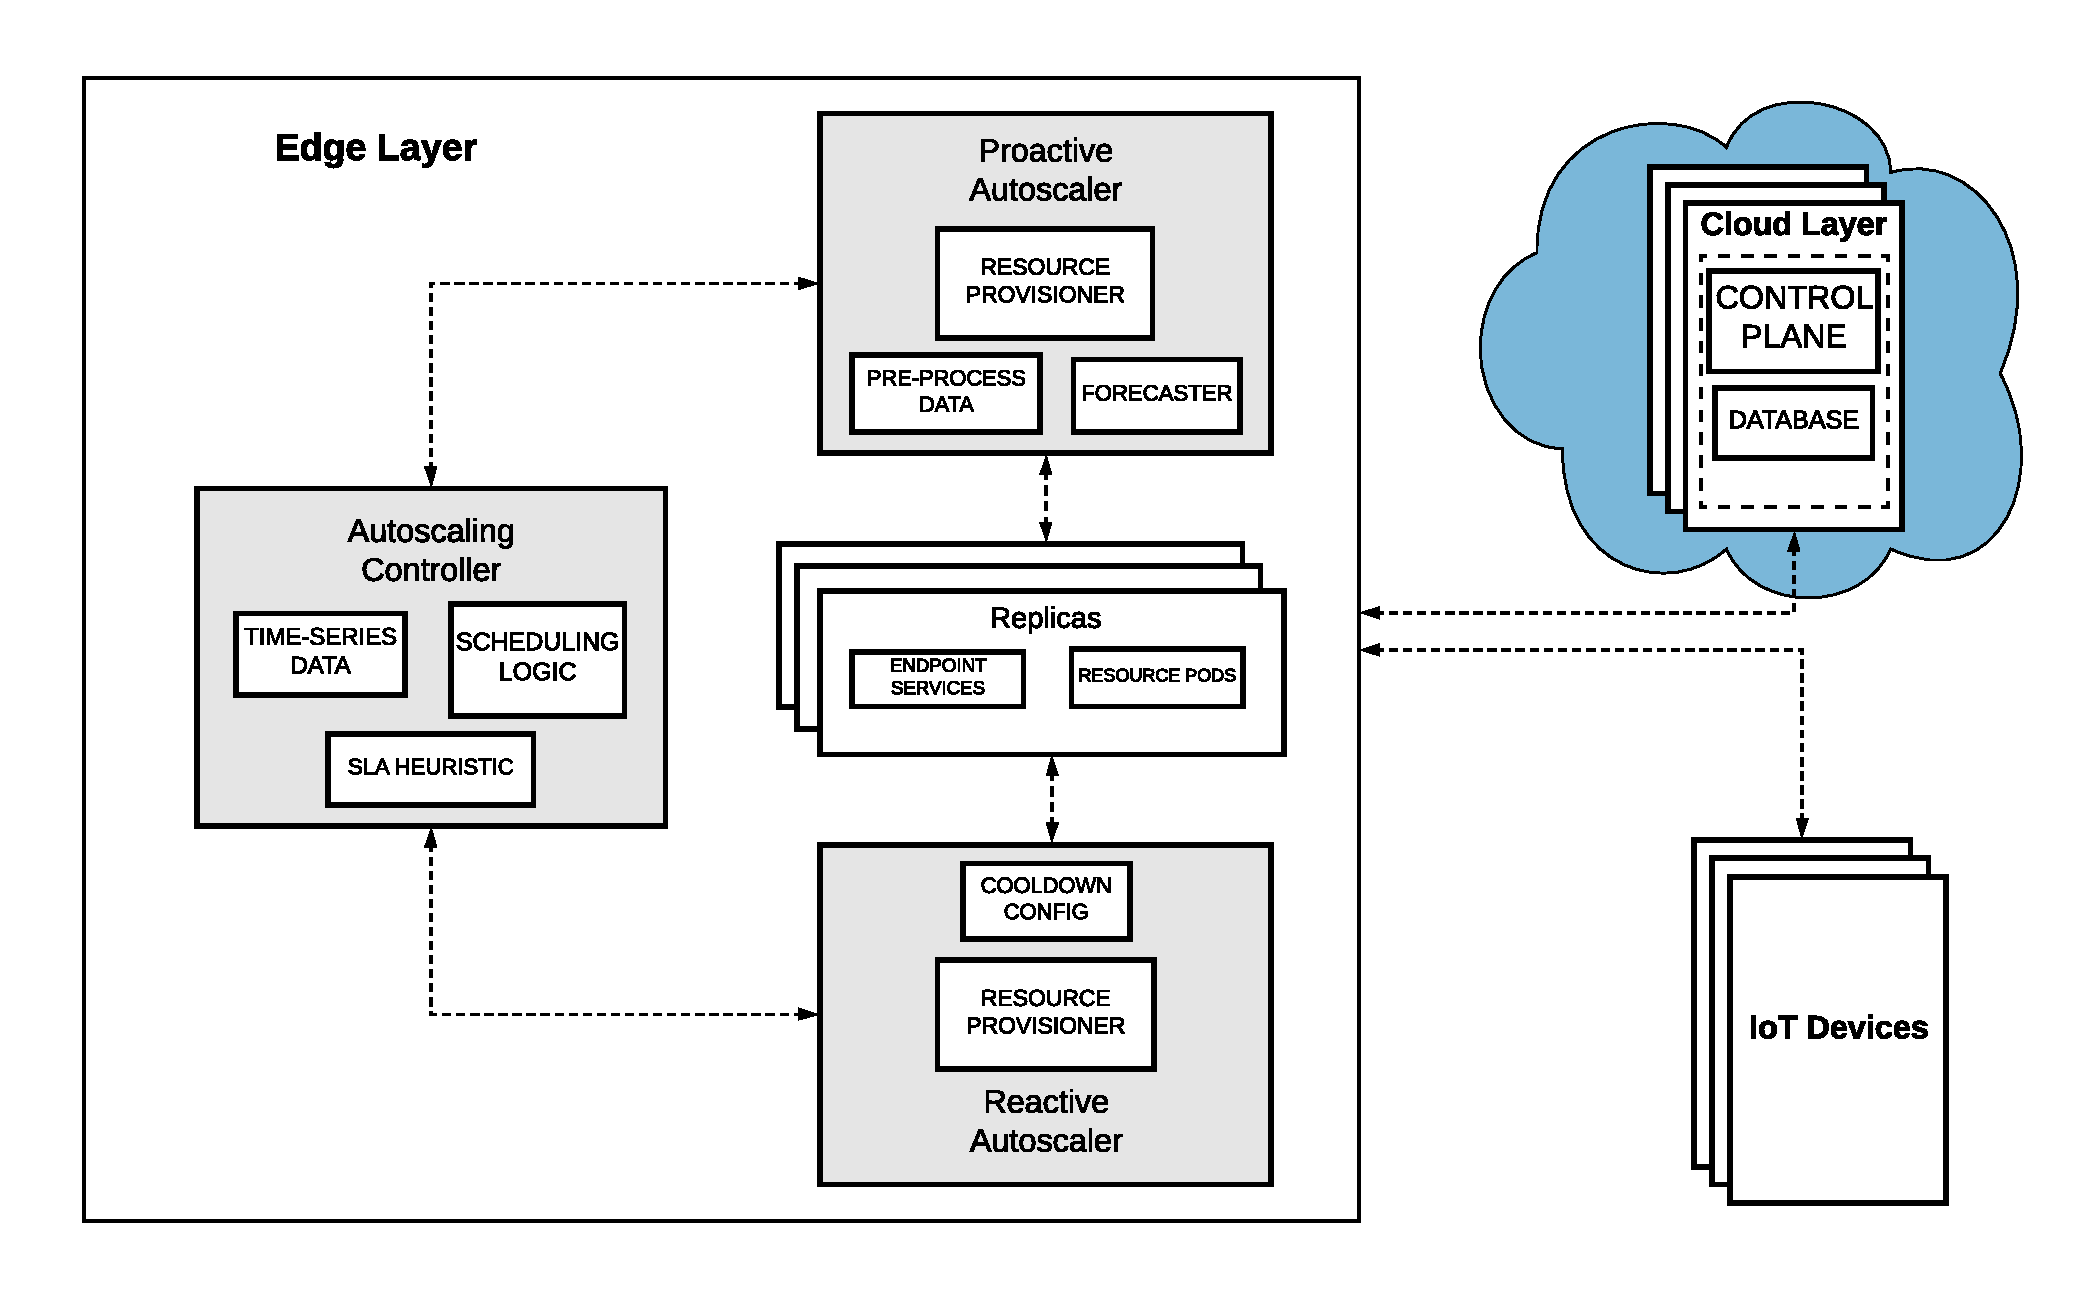
\includegraphics[width=1.0\linewidth]{Figures/Hybrid-Architecture-Overview.pdf}
    \label{fig:hybrid-arch-overview}
\end{figure}

An overview of the hybrid autoscaler architecture is shown in Figure~\ref{fig:hybrid-arch-overview}. The overall architecture is formulated using a hierarchical model as described in Section~\ref{sec:ch3-edge-implementation}. The edge node consists of three main sections. The first is the reactive auto-scaling subsystem, which has the resource provisioning module, and the configuration which dictates the cooldown logic for scaling up and down. As Zhang \textit{et al}.~\cite{zhang2019quantifying} demonstrated, the micro-service system stability is directly related to the careful selection of cool-down parameters. Thus, these must be available to the user in a configuration setting.\par

The second subsystem is the proactive autoscaler. From a high-level perspective, there are three main components. The resource provisioning module is similar to that of the reactive autoscaler, however, it also consists of a forecaster using a deep-learning-based machine learning model, and a data pre-processing algorithm. The data pre-processing algorithm removes any noise present in the time series data, and smoothens the data curves, making it easier for the forecaster to make predictions in a low-cost manner. A detailed implementation of the forecaster logic itself will be discussed in Section~\ref{subsec:ch5-proactive-auto-subsection}.\par

Finally, the auto-scaling controller determines which auto-scaling logic will be applied to the replicas, and also keeps track of any SLA violations. It also hosts the time-series metric data and has a feedback loop with the proactive autoscaler. If it detects any SLA violations were caused after auto-scaling during a configured time window, it automatically adjusts the hyper-parameters of the proactive forecaster in an attempt to predict from the time-series data more accurately during the next training iteration. Correspondingly, a lack of SLA violations during a specific time window period reverts the autoscaler parameters back to the original values, in an attempt to streamline the training process further. Such a heuristic method allows for the freeing up of the complex hyper-parameter tuning process seen in most proactive models from the autoscaler deployment process. This is a key part of the architecture which is essential in answering the research questions outlined in the thesis.\par


\subsection{Autoscaler Subsystems}
\label{subsec:ch4-hybrid-arch}

At a high level, a container orchestration's default horizontal pod autoscaler operates on the ratio between the current and desired metric values, which can be written as:

\begin{equation}
    replicas_{desired} = \lceil replicas_{current} \times \cfrac{metric_{current}}{metric_{desired}}\rceil
    \label{eqn:replica-desired}
\end{equation}

For example, for a given deployment with a current replica count as 1, if the desired metric value is 50 resource units, and the current value is 100, then the number of desired replicas will be $\lceil 1 \times \cfrac{100}{50}\rceil = 2$. There are three other important parameters that are key to controlling the process of horizontal pod scaling, namely ``tolerance'', ``scale up cooldown'', and ``scaledown cooldown''.\par

The tolerance is a constant which informs the autoscaler when to skip calculating new replicas. The tolerance ratio can be calculated as:

\begin{equation}
    \label{eqn:tolerance}
    tolerance = \abs{ \cfrac{metric_{desired} - metric_{current}}{metric_{desired}} }
\end{equation}

For example, if the current metric is 60, and the desired metric is 50, the tolerance is calculated as $ tolerance = \abs{ \cfrac{60 - 50}{60}} = 0.167$. By default, if the tolerance value is below 0.1, autoscaling is skipped for that control loop, however, this can be configured by the user.\par

The scale-up and scale-down cooldowns control how quickly auto-scaling occurs. The default approach which is set by the container orchestration can be concisely stated as ``Scale up as quickly as possible, while scaling down very gradually.'' Therefore, the default scale-up cooldown is set to 0 seconds, meaning that the moment the desired replica value increases, the autoscaling will be initiated. However, the default cooldown is set to 300 seconds, meaning that if the desired replica value is decreased, it must remain decreased for 300 seconds (or 20 control loops) before the resources are scaled down.\par

A cooldown value that is too low would cause a repetitive scaling up and scaling down of the resources, leading to significant stress on the system as well as wastage of resources. Meanwhile, a large value would render the autoscaler unable to assign resources quickly enough to ensure SLA latency compliance. Thus, for the proposed autoscaler, the default values are modified to ensure that a moderate cooldown value was chosen to ensure the best system stability and SLA compliance. This cooldown configuration would be applied to both the proactive and reactive auto-scaling subsystems to maintain consistency.\par

For auto-scaling proactively, a custom metric $metric_{forecast}$ is used, which defines the future CPU workload expected to be exerted on the micro-service application $\mathcal{T}$ seconds in the future, where $\mathcal{T}$ can be configured during the autoscaler deployment process. This $metric_{forecast}$ value will be sent to the auto-scaling controller by the proactive autoscaler.\par

\subsubsection{Scheduler}

The autoscaler controller consists of a scheduling logic module which handles when to switch between proactive and reactive auto-scaling. Algorithm~\ref{alg:scheduling-logic-daemon} explains how the hybrid scheduling logic determines which auto-scaling subsystem to employ. The hybrid scheduler takes four inputs, namely the $replicas_{current}$, $metric_{current}$, $metric_{desired}$, and $metric_{forecast}$ variables discussed above. It outputs one value, the $replicas_{desired}$.\par

The autoscaler computes two replica values, one for the proactive forecaster which determines the replicas after $\mathcal{T}$ seconds, and one for the reactive forecaster, which determines the current resource requirements. By computing the future requirements $replicas_{forecast}$ using Equation~\ref{eqn:replica-desired}, if it is found that this requirement is higher than the current resource requirement $replicas_{current}$, then the hybrid scheduler outputs the forecaster replica count as the desired replicas. Otherwise, the hybrid scheduler determines that the utilization is either stabilizing or about to decline. Due to this, it makes a decision that the reactive replica count $replicas_{reactive}$ is the desired number. The hybrid scheduler then sends this value to the container orchestration controller plane to autoscale the replicas accordingly using either the reactive or proactive sub-system's resource provisioning modules.\par

%TC:ignore
\begin{algorithm}
    \caption{Scheduler algorithm}
    \label{alg:scheduling-logic-daemon}
    \textbf{Input}: $replicas_{current},\, metric_{current},\, metric_{desired},\, metric_{forecast}$\\
    \textbf{Output}: $replicas_{desired}$
    \begin{algorithmic}
        \State $replicas_{forecast} \gets \lceil replicas_{current} \times \cfrac{metric_{forecast}}{metric_{desired}}\rceil$
        \State $replicas_{reactive} \gets \lceil replicas_{current} \times \cfrac{metric_{current}}{metric_{desired}}\rceil$
        \If{$replicas_{forecast} > replicas_{reactive}$}
            \State $replicas_{desired} \gets replicas_{forecast}$
        \Else
            \State $replicas_{desired} \gets replicas_{reactive}$
        \EndIf
        \State \Return $replicas_{desired}$
    \end{algorithmic}
\end{algorithm}
%TC:endignore

\subsubsection{Reactive Resource Provisioning}

The reactive autoscaler subsystem is responsible for determining whether or not auto-scaling should proceed based on the given configuration. The reactive algorithm's resource provisioning is built on top of the default horizontal pod autoscaler deployed by the Kubernetes container orchestration platform. The autoscaler is modified in such a way that it has its cooldown parameters set to a moderate value to ensure adaptability to SLA-constrained scenarios, while also maintaining system stability. The workflow is shown below in Algorithm~\ref{alg:reactive-resource-provision}. The algorithm takes the current metric value as an input, as well as the desired metric value, and outputs the decision to autoscale or not. It does this by computing the $tolerance$ value as shown in Equation~\ref{eqn:tolerance}. If this tolerance is above the configured threshold, the autoscaler will modify the replicas, otherwise, it will ignore the current auto-scaling request.\par

%TC:ignore
\begin{algorithm}
    \caption{Reactive resource provisioning}
    \label{alg:reactive-resource-provision}
    \textbf{Input}: $metric_{current},\, metric_{desired}$\\
    \textbf{Output}: $autoscale$
    \begin{algorithmic}
        \State $tolerance \gets \abs{ \cfrac{metric_{desired} - metric_{current}}{metric_{desired}} }$
        \If{$tolerance > \gamma$}
            \State $autoscale \gets Yes$
        \Else
            \State $autoscale \gets No$
        \EndIf
        \State \Return $autoscale$
    \end{algorithmic}
\end{algorithm}
%TC:endignore

\subsubsection{Data Pre-Processor}
\label{subsubsec:ch4-data-pre-process}

\begin{figure}[htb]
    \centering
    \caption[Pre-processing of data]{Pre-processing of data, source:~\cite{comsolcurvefitting}}
    \label{fig:data-pre-process}
    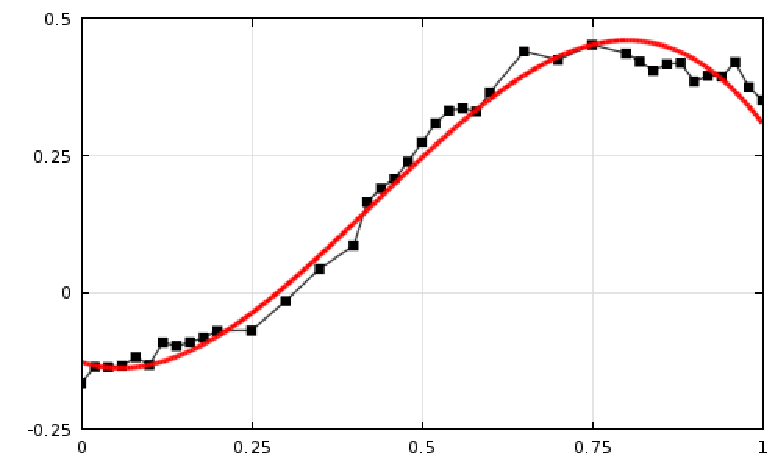
\includegraphics[width=0.6\linewidth]{Figures/Data-Pre-Processing.pdf}
\end{figure}

To speed up the forecast process even further and reduce the resource and time requirements, the time-series data can be pre-processed to smoothen it. Doing so makes it easier for the deep learning model to extract patterns, and reduces the training and validation loss. Figure~\ref{fig:data-pre-process} shows a graph containing raw input (shown in black), and a smoothened data curve (shown in red). While the red curve contains all the requisite information of the data (such as the slope of the curve, maximum and minimum value, etc.), it removes the noise, reducing the overall loss, and reducing the length of the training window data sequence the LSTM requires to accurately predict future data.\par

\subsubsection{Proactive Forecaster}

The forecaster portion of the autoscaler is used to generate this $metric_{forecast}$ value. The autoscaler controller periodically scrapes the windowed data stored in the cloud database to keep a form of cached time-series workload. It combines this workload with the future workload $metric_{forecast}$. To do so, the controller requests the $metric_{forecast}$ value for a specified time $\mathcal{T}$ from the proactive forecaster, and the forecaster then sends this value back after pre-processing the scraped data and training the forecaster model.\par

Several time series forecaster algorithms exist, with the two prominent ones being the more modern deep learning algorithm LSTM, and the traditional deep learning algorithm ARIMA. Siami-Namini \textit{et al}.~\cite{siami2018comparison} demonstrated that LSTM implementations outperformed ARIMA, reducing error rates by over 80\%. Furthermore, they were able to demonstrate that the number of deep learning ``epochs'', or the total amount of training time required for LSTM did not need to be set to a high value. In fact, setting a significantly higher value than required was shown to degrade performance due to over-fitting. The authors posited that LSTM worked so well due to the ``rolling updates'' being performed on the model. The LSTM weights are only set once when the forecaster is deployed, after which they are always updated on every call of the training algorithm, meaning there is a continuous improvement to the prediction results.\par

Based on the investigations above, it was determined that LSTM time-series forecasters would be ideally suited for a proactive autoscaler designed for the hybrid autoscaler architecture. Algorithm~\ref{alg:proactive-forecast-alg} shows the implementation of such a forecaster. The autoscaler controller implements a control loop every $\mathcal{P}$ seconds, where it requests the latest time-series metric prediction from the forecaster. As input, the algorithm takes the variable $lookback$, which is the number of data points it should use as a window to train, the training iteration count $epochs$, and the $learning\_rate$, which determines the step size per each training iteration moving towards the minimum loss value. The forecaster then pre-processes this data to remove the noise as shown above in Section~\ref{subsubsec:ch4-data-pre-process}, and performs a training iteration using the configured hyper-parameters. It then computes the validation loss, and accepts this model as the most accurate one if it has a lower validation loss than the previous training iterations. Otherwise, the current model is rejected and the forecaster uses the older model instead. Finally, the model predicts the future metric and returns it to the autoscaler controller for determining the auto-scaling based on Algorithm~\ref{alg:scheduling-logic-daemon}.\par


\begin{algorithm}
    \caption{Proactive forecaster}
    \label{alg:proactive-forecast-alg}
    \textbf{Input}: $lookback \geq 0, 0 \leq epochs \leq 100, 0 \leq learning\_rate \leq 1$\\
    \textbf{Output}: $metric_{forecast}$
    \begin{algorithmic}
        \State $lstm\_model \gets lstm.initialize()$
        \State $time\_series \gets get\_latest\_data()$
        \State $lstm\_input \gets get\_input(time\_series\_data, lookback)$
        \State $lstm\_input \gets preprocess\_data(lstm\_input)$
        \State $new\_model \gets train(lstm\_input, epochs, learning\_rate)$
        \If{$validation\_loss(new\_model) < validation\_loss(lstm\_model)$}
            \State $lstm\_model \gets new\_model$
        \EndIf
        \State $metric_{forecast} \gets lstm\_model.predict(lstm\_input)$
        \State \Return $metric_{forecast}$
    \end{algorithmic}
\end{algorithm}

\subsubsection{Proactive Resource Provisioning}

The proactive subsystem's resource provisioning module works in a similar manner to the reactive autoscaler. If the autoscaler controller's scheduling logic determines that a proactive auto-scaling must take place, it requests the cloud layer to proceed with auto-scaling using the proactive subsystem's resource provisioning, which is shown in Algorithm~\ref{alg:proactive-resource-provision}. The algorithm takes the desired and forecast metric values as input and outputs the decision to autoscale or not. It does this by computing the $tolerance$ value as shown in Equation~\ref{eqn:tolerance}. If this tolerance is above the configured threshold, the autoscaler will modify the replicas, otherwise, it will ignore the current auto-scaling request.\par

\begin{algorithm}
    \caption{Proactive resource provisioning}
    \label{alg:proactive-resource-provision}
    \textbf{Input}: $metric_{forecast},\, metric_{desired}$\\
    \textbf{Output}: $autoscale$
    \begin{algorithmic}
        \State $tolerance \gets \abs{ \cfrac{metric_{desired} - metric_{forecast}}{metric_{desired}} }$
        \If{$tolerance > \gamma$}
            \State $autoscale \gets Yes$
        \Else
            \State $autoscale \gets No$
        \EndIf
        \State \Return $autoscale$
    \end{algorithmic}
\end{algorithm}

\subsubsection{SLA Heuristic Feedback}

Finally, the last hybrid autoscaler module is the autoscaler controller's SLA-based heuristic feedback loop, which assists the proactive forecaster in increasing its prediction accuracy. The autoscaler constantly checks for SLA violations in the edge deployment using a control loop. Typically, the SLA checks are done for a sufficiently lengthy period of time such as one day. If an SLA violation is found, it is concluded that the application was unable to autoscale quickly enough to avoid the cold start problem. This could be due to a number of causes, such as insufficient training data, or the LSTM hyper-parameters being too conservative. To temporarily boost learning, the controller then decreases the learning rate to increase the probability of the model escaping from the local minima to find the global one, increases the batch size to reduce under-fitting, and increases the number of epochs to reduce loss. All these parameters have a threshold, as increasing or decreasing certain parameters by a large amount may lead to issues such as over-fitting or infeasibly lengthy training times.\par

\begin{algorithm}
    \caption{SLA-based heuristic feedback}
    \label{alg:sla-heuristic-feedback}
    \textbf{Input}: $\mathcal{V},\,learning\_rate,\,batch\_size,\,epochs$\\
    \textbf{Output}: $hyperparameters_{modified}$
    \begin{algorithmic}
        \State $initial\_rate \gets learning\_rate$
        \State $initial\_batch \gets batch\_size$
        \State $initial\_epochs \gets epochs$
        \If{$\mathcal{V}$ > 0}
            \State $batch\_size \gets MAX(batch\_size + \alpha, \mathcal{A})$
            \State $learning\_rate \gets MIN(learning\_rate - \beta, \mathcal{B})$
            \State $epochs \gets MIN(epochs - \lambda, \mathcal{L})$
        \Else
            \State $epochs \gets initial\_epochs$
            \State $learning\_rate \gets initial\_rate$
            \State $batch\_size \gets initial\_batch$
        \EndIf
        \State $hyperparameters_{modified} \gets (learning\_rate, batch\_size, epochs)$
        \State \Return $hyperparameters_{modified}$
    \end{algorithmic}
\end{algorithm}

Finally, if the feedback control loop discovers that no SLA-violations occurred during the time-period, it concludes that the LSTM has sufficiently learned the primary characteristics of the time-series. As discussed by Siami-Namini \textit{et al}.~\cite{siami2018comparison}, the ``rolling-updates'' feature of LSTM allows the autoscaler to safely reset the hyper-parameters of the model, while preserving the learning and weights of the previous rounds of training. Algorithm~\ref{alg:sla-heuristic-feedback} shows how the heuristic feedback is set up. The algorithm takes the three hyper-parameters of the LSTM, namely $learning\_rate$, $batch\_size$, and $epochs$, along with the $\mathcal{V}$ which stores the number of SLA violations that occurred during a specified time window. Using these parameters, the algorithm computes the new LSTM hyper-parameters and outputs them to the proactive forecaster to use in the next training cycle.\par

\subsection{Computational Complexity Analysis}
\label{subsec:ch4-space-time-comp}

To analyze the space and time complexity of the auto-scaling architecture, some simplifying assumptions must be made. Firstly, the complexities will be for one control loop of the container orchestration platform. By default, controller orchestration platforms have control loops which are executed every 15 seconds. During each of these loops, auto-scaling is assessed and implemented. Thus we will ignore the complexities involved in the control loop itself, and focus only on the autoscaler.\par

Secondly, for the proactive forecaster, the complexities of the LSTM are simplified to the basic multiplicative steps involved in the training step. Other internal logic such as the $\sigma$ function is assumed to have $\mathcal{O}(1)$ space and time complexity.\par

Finally, assuming the hybrid autoscaler $\mathcal{H}$ takes a time-series data of length $\mathcal{N}$, it stores this data in an array data structure. The rest of the inputs can be considered as single variables. The forecaster's LSTM weights are assumed to be a two-dimensional matrix of size $A \times B$. Thus the space complexity can be easily computed for this information. The variables each have a space complexity of $O(1)$. Meanwhile, the time-series array has a complexity of $\mathcal{O}(N)$, and the weights are of complexity $\mathcal{O}(N^2)$. Thus, the space complexity can be written as the sum of the two values and simplified.

\[Complexity_{space}(\mathcal{H}) = \mathcal{O}(N^2) + \mathcal{O}(N) + \mathcal{O}(1)\]
\begin{equation}
    \Rightarrow Complexity_{space}(\mathcal{H}) = \mathcal{O}(N^2)
\end{equation}

The time complexity is a more complex calculation. The complexities of the reactive autoscaler, proactive autoscaler, and autoscaler controller need to be computed. The autoscaler controller only stores the time-series array and computes the new hyper-parameters in Algorithm~\ref{alg:sla-heuristic-feedback}. Both of these operations can be completed in constant time, thus the time complexity for the controller is as follows:

\begin{equation}
    Complexity_{time}(controller) = \mathcal{O}(1)
\end{equation}

Similarly, the reactive autoscaler only computes the tolerance value, which is also a constant operation independent of data size, thus the time complexity can be written as:

\begin{equation}
    Complexity_{time}(reactive) = \mathcal{O}(1)
\end{equation}

For the proactive autoscaler, the forecaster internally computes matrix multiplications, such as of the various LSTM weights and vectors. For example, Equation~\ref{eqn:input-gate} can be rewritten as follows.

\begin{equation}
    i_{t} = \sigma(W_{i}(x) \cdot x_{t} + W_{i}(h) \cdot h_{t-1} + b_{i})
\end{equation}

In the above equation, we assume the dimension of the variables as follows:

\begin{itemize}
    \item $W_{i}(x) \in \R^{m \times n}$
    \item $x_{t} \in \R^{n}$
    \item $W_{i}(h) \in \R^{m \times m}$
    \item $b_{i} \in \R^{m}$
    \item $h_{t-1} \in \R^{m}$
\end{itemize}

Using these values, the time complexity of each of the individual multiplicative and additive operations can be computed.

\[Complexity_{time}(W_{i}(x) \cdot x_{t}) = \mathcal{O}(mn)\]
\[Complexity_{time}(W_{i}(h) \cdot h_{t-1}) = \mathcal{O}(m^2)\]
\begin{equation}
    Complexity_{time}(W_{i} \cdot [x_{t}, h_{t-1}] + b_{i}) = \mathcal{O}(mn + m^2 + m)
\end{equation}

Therefore the complexity of the proactive component can be written as:

\[Complexity_{time}(proactive) = \mathcal{O}(mn + m^2 + m)\]
\[\Rightarrow Complexity_{time}(proactive) = \mathcal{O}(m \times (m + n + 1))\]
\begin{equation}
    \Rightarrow Complexity_{time}(proactive) = \mathcal{O}(N^2)
\end{equation}

This is the value of one training epoch. For an LSTM training process with $\tau$ training epochs, the complexity becomes $\mathcal{O}(\tau N^2)$. However, it is important to note that the value of $\tau$ is a constant, thus the final proactive complexity can be reduced back to $\mathcal{O}(N^2)$.\par

Combining the time complexities of all three hybrid components, the final complexity for the hybrid autoscaler $\mathcal{H}$ can be re-written as:

\[Complexity_{time}(\mathcal{H}) = \mathcal{O}(1) +  \mathcal{O}(1) + \mathcal{O}(N^2)\]

\begin{equation}
    \label{eqn:hybrid-time-complexity}
    \Rightarrow Complexity_{time}(\mathcal{H}) = \mathcal{O}(N^2)
\end{equation}

From the results in Equation~\ref{eqn:hybrid-time-complexity}, it is clear that the hybrid algorithm performs extremely well in a polynomial time complexity. Even though it is shown that no mathematically certain decision can be computed in a polynomial time due to the NP-Hard nature of the problem statement, the hybrid algorithm is proven to provide an alternative that is able to approximate a high accuracy auto-scaling decision in polynomial time.